% --------------------------- REX
\section{Retour d'Expérience (REX)} % --------------------------- REX
% --------------------------- REX

\subsection{Spécifications fonctionnelles}

\subsubsection{Cas d’utilisations}

% #############################################
\noindent\textsc{\bf{A1 - UC1 :} Consulter une prestation de maintenance}
\begin{shaded}
\noindent\textsc{Résumé :}\\

Pendant une intervention, le technicien souhaite accède à l’historique du dossier pour une prestation de maintenance donné. \\

\noindent\textsc{Utilisateur :}\\

Technicien ou Responsable d’affaires ou Commercial \\

\noindent\textsc{Scénario :} \\
\begin{enumerate}
    \item   L’utilisateur fait une recherche avec la référence d’un contrat ou le nom d’une société
    \item   Le système affiche la liste des contrats pouvant correspondre
    \item   L’utilisateur sélectionne son contrat
    \item   Le système affiche l’état actuel du contrat avec la liste des commandes
    \item   L’utilisateur sélectionne la commande correspondant à son intervention
    \item   Le système affiche l’état actuel de la commande avec la liste des prestations de maintenance
    \item   L’utilisateur sélectionne la prestation de maintenance correspondant à l’intervention
    \item   Le système retourne la prestation de maintenance et les pièces jointes qui lui sont associées \\
\end{enumerate}
\noindent\textsc{Scénarii alternatifs :} \\
\begin{enumerate}
    \item L’utilisateur fait une recherche avec la référence de la commande
    \begin{enumerate}
        \item Le système affiche la liste des commandes pouvant correspondre à la recherche
        \item On reprend le scénario nominal à l’étape de 5 \\
    \end{enumerate}
    \item L’utilisateur fait une recherche avec la référence de la prestation de maintenance
    \begin{enumerate}
        \item Le système affiche la liste des prestations de maintenance pouvant correspondre à la recherche
        \item On reprend le scénario nominal à l’étape 7
    \end{enumerate}
\end{enumerate}
\end{shaded}
% #############################################
\noindent\textsc{\bf{A1 - UC2 :} Saisir le retour d’expérience}
\begin{shaded}
\noindent\textsc{Résumé :}\\

Après une prestation de maintenance effectuée par un technicien, il peut rentrer un résumé et les détails sur cette dernière dans une base de connaissance. \\

\noindent\textsc{Utilisateur :} \\

Technicien \\

\noindent\textsc{Scénario :} \\
\begin{enumerate}
    \item L’utilisateur consulte une prestation de maintenance (A1 - UC1) et demande une saisie de retour d’expérience
    \item Le système demande à l’utilisateur de saisir les informations sur son retour d’expérience
    \item L’utilisateur renseigne les différents champs et valide la saisie
    \item Le système l’enregistre et affiche le résultat de sa saisie \\
\end{enumerate}
\end{shaded}
% #############################################
\noindent\textsc{\bf{A1 - UC3 :} Associer des pièces jointes au retour d’expérience}
\begin{shaded}
\noindent\textsc{Résumé :}\\

L’utilisateur veut associer des pièces jointes de différentes catégories à la prestation de maintenance. \\

\noindent\textsc{Utilisateur :} \\

Technicien \\

\noindent\textsc{Scénario :} \\
\begin{enumerate}
    \item L’utilisateur consulte une prestation de maintenance (A1 - UC1) et demande l’ajout de pièces jointes
    \item L’utilisateur choisit les pièces jointes qu’il veut associer au dossier et leur affecte une catégorie
    \item Les pièces jointes sont récupérées depuis le média qu’il utilise (tablette, ordinateur, etc.)
\end{enumerate}

\end{shaded}

\subsubsection{Services}

\begin{description}
    \item[\textbullet] Rechercher un contrat par référence (identifiant unique) \\
        \it{Description succincte :} ce service permet de récupérer un contrat en utilisant sa référence pour effectuer la recherche. \\
        \it{Complexité\footnote{On évalue la complexité d’un service sur une échelle à trois valeurs : \bf{simple}, \bf{moyen}, \bf{complexe}} :} \bf{simple}.
    \item[\textbullet] Rechercher un contrat par le nom de la société dans lequel il intervient \\
        \it{Description succincte :} ce service permet de récupérer un contrat en utilisant le nom de la société pour effectuer la recherche. \\
        \it{Complexité :} \bf{simple}.
    \item[\textbullet] Récupérer les commandes associées à une référence d’un contrat  \\
        \it{Description succincte :} ce service permet de récupérer les commandes associées à un contrat en utilisant la référence de ce dernier. \\
        \it{Complexité :} \bf{simple}.
    \item[\textbullet] Rechercher une commande par sa référence \\
        \it{Description succincte :} ce service permet de récupérer une commande en utilisant sa référence. \\
        \it{Complexité :} \bf{simple}.
    \item[\textbullet] Récupérer les prestations de maintenance associées à une référence d’une commande \\
        \it{Description succincte :} ce service permet de récupérer les prestations de maintenance en utilisant la référence de la commande associée  \\
        \it{Complexité :} \bf{simple}. 
    \item[\textbullet] Rechercher une prestation de maintenance par sa référence \\
        \it{Description succincte :} ce service permet de récupérer une prestation de maintenance en utilisant sa référence. \\
        \it{Complexité :} \bf{simple}.
    \item[\textbullet] Mise à jour d’une prestation de maintenance \\
        \it{Description succincte :} ce service permet la mise à jour d’une prestation de maintenance en exploitant les saisies de l’utilisateur. \\
        \it{Complexité :} \bf{moyen}.
    \item[\textbullet] Ajouter un document à la prestation de maintenance \\
        \it{Description succincte :} ce service permet de téléverser un document et de l’associer à une prestation de maintenance. \\
        \it{Complexité :} \bf{moyen}.
\end{description}

\subsubsection{Identification du bloc applicatif}

Les services dégagés précédemment répondant à un axe d’amélioration commun, concernant les retours d’expérience, un nouveau bloc applicatif apparaît. Intitulé “Outil REX”, ce bloc permet de regrouper les différents services répondant aux cas d’utilisation liés aux retours d’expérience. Ces cas d’utilisation nécessitant de communiquer avec la base de données, un acteur supplémentaire se doit alors d’être ajouté, comme représenté sur le schéma ci-dessous.

\begin{figure}[H]
    \label{fig-uc-rex}
    \noindent\makebox[\textwidth]{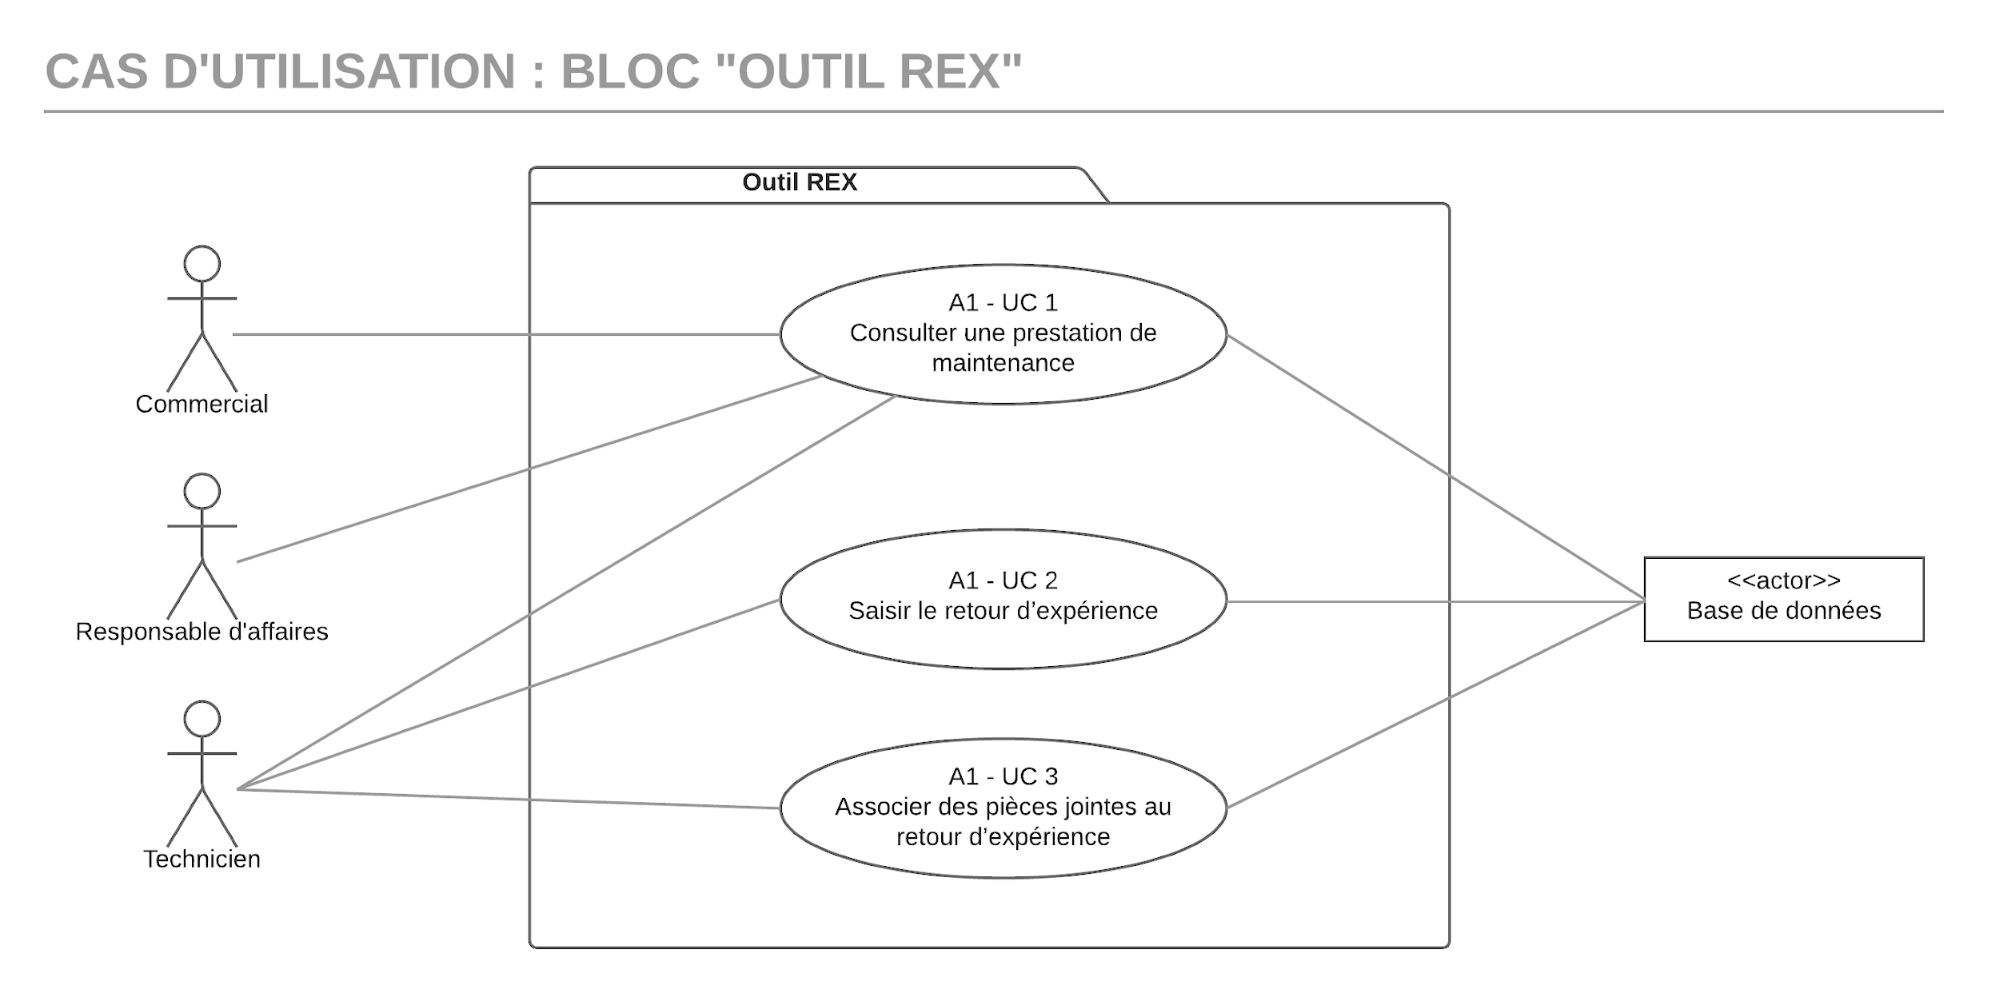
\includegraphics[width=12cm]{figures/uc_bloc_rex.png}}
    \caption{Diagramme des cas d'utilisation de l'outil REX}
\end{figure}

Le bloc “Outil REX” utilisant les données relatives aux contrats de maintenance, une communication depuis le bloc applicatif “ADV” est nécessaire. De même, l’accès aux informations reliées aux prestations de maintenance étant nécessaire pour renseigner les retours d’expérience, un transfert de données depuis le bloc “CLARIFY” est également présent. Enfin, les retours d’expériences concernent à la fois les techniciens qui les saisissent suite à leurs prestations de maintenance, mais également les commerciaux et les responsables d’affaires qui souhaitent suivre les informations disponibles sur les retours d’expérience. De fait, une communication avec le bloc “People Soft” et “SUPRA” est également nécessaire.

\begin{figure}[H]
    \label{fig-dep-rex}
    \noindent\makebox[\textwidth]{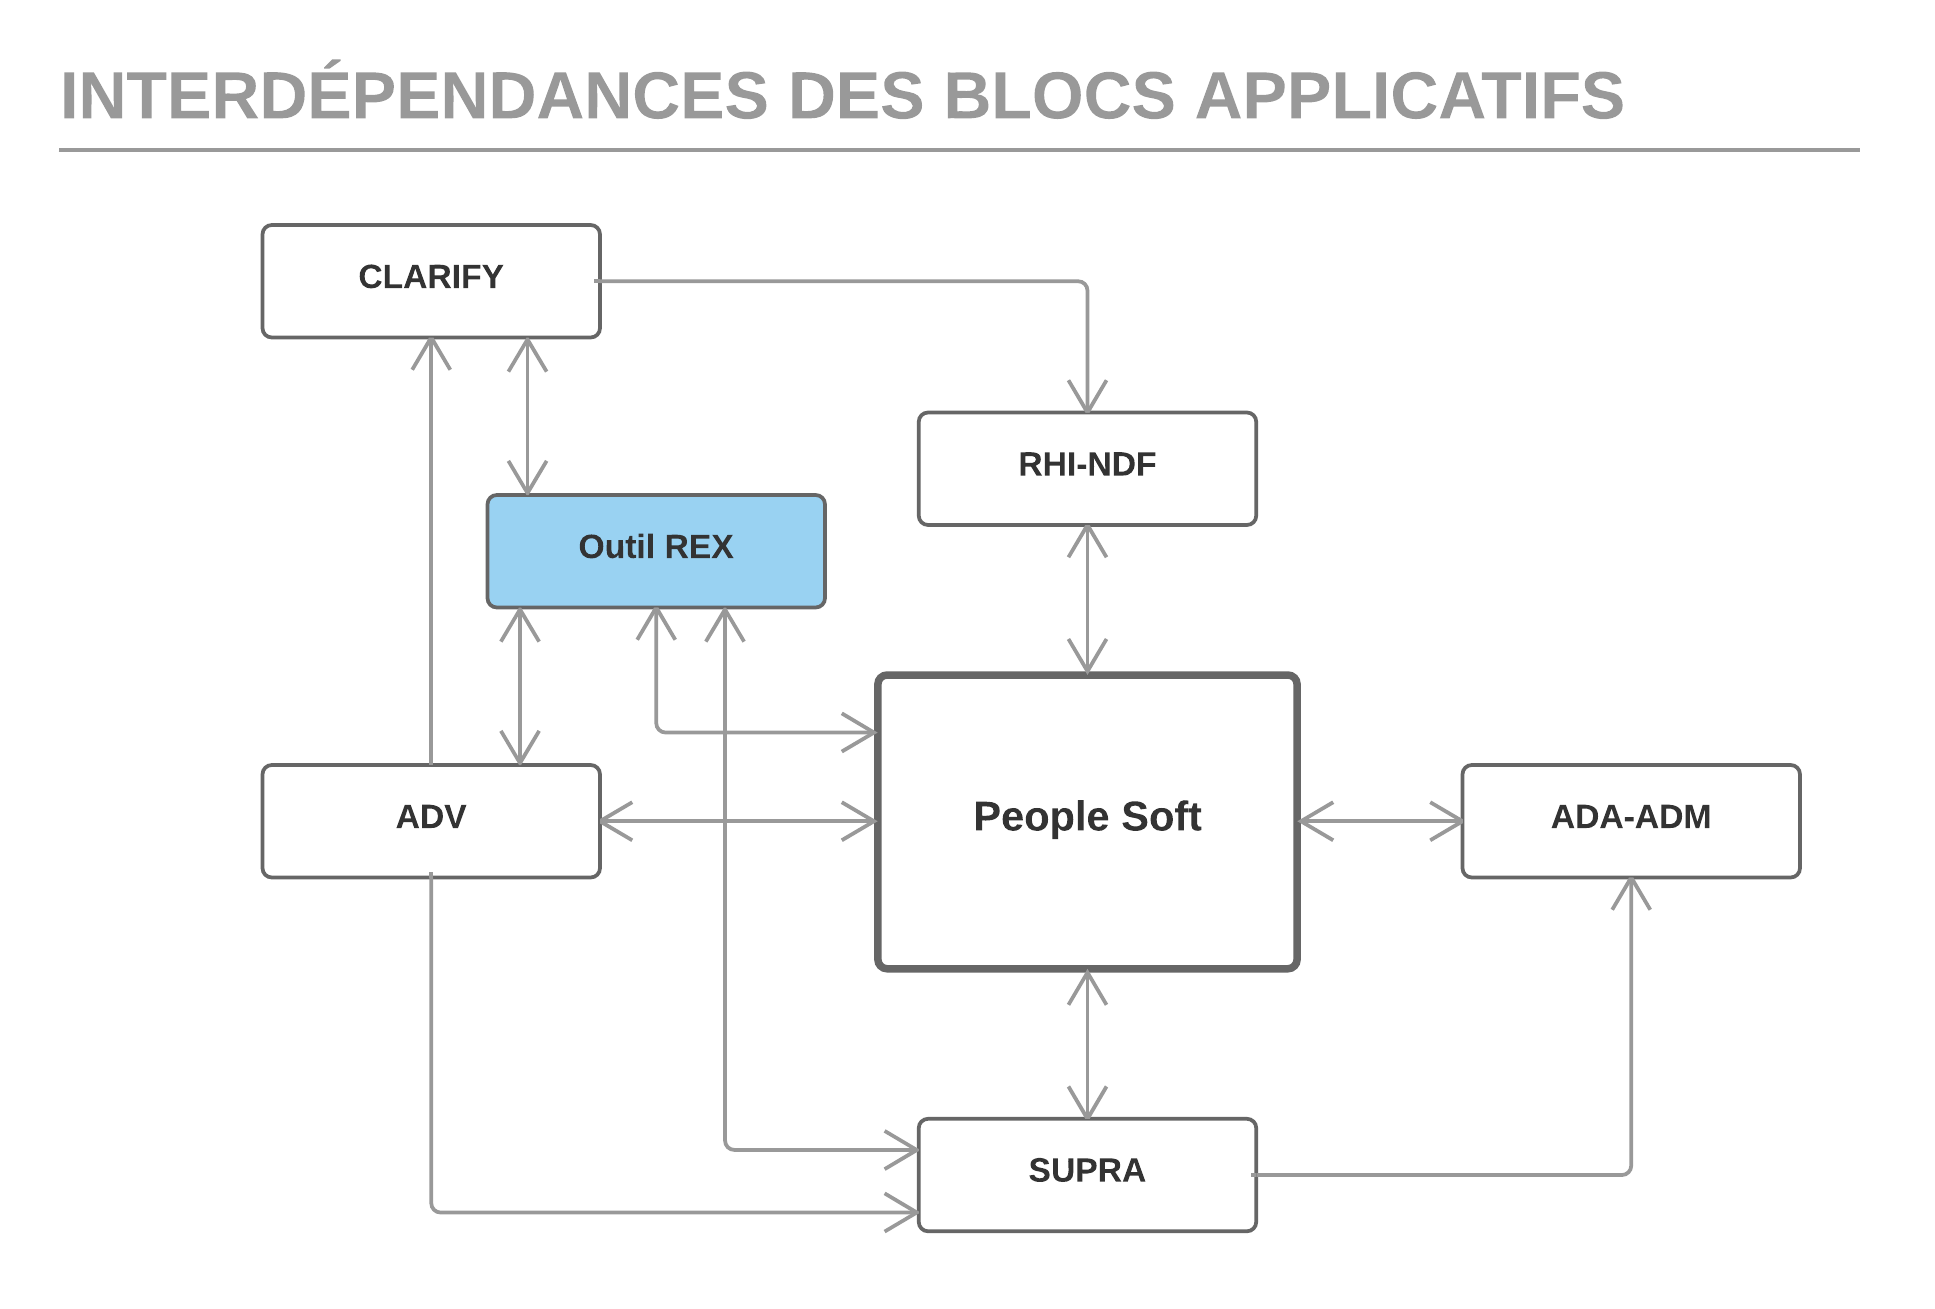
\includegraphics[width=12cm]{figures/dependances_bloc_rex.png}}
    \caption{Schéma des interdépendances de l'outil REX}
\end{figure}

\subsection{Gestion des données}

\subsubsection{Objets métiers}

Les différents cas d’utilisation décrits précédemment permettent d’identifier les objets métiers qui sont concernés par ceux-ci, permettant dans le même temps de compléter le modèle conceptuel de données correspondant à la solution spécifique proposée.

\begin{table}[H]
    \begin{tabular}{p{3cm}|p{10cm}|p{3cm}}
    Objet métier & Description & Cas d'utilisations \\ \hline
    Contrat & Contrat de maintenance signé par un client de SPIE Sud-Est & A1-UC1 ; A1-UC2 ; A1-UC3 \\ \hline
    Commande & Commande de la part d’un client d’un ensemble de prestations de maintenance, dans le cadre d’un contrat de maintenance & A1-UC1 ; A1-UC2 ; A1-UC3 \\ \hline
    Prestation de maintenance & Intervention de maintenance effectuée par un technicien pour un client & A1-UC1 ; A1-UC2 ; A1-UC3 \\ \hline
    Retour d’expérience & Compte-rendu effectué par un technicien après une intervention de maintenance & A1-UC2 ; A1-UC3 \\ \hline
    Document & Document numérique pouvant être associé à une prestation de maintenance comme étant une pièce jointe & A1-UC1 ;
A1-UC3 \\
    Technicien & Technicien réalisant les prestations de maintenance & A1-UC1 ; A1-UC2 ; A1-UC3 \\ \hline
    Commercial & Commercial signant les contrats de maintenance & A1-UC1 \\ \hline
    Responsable d’affaires & Responsable d’affaires suivant le déroulement des contrats de maintenance & A1-UC1 \\
    \end{tabular}
    \caption{Tableau des Objets Métiers pour l'Outil REX}
\end{table}

Le bloc applicatif “Outil REX” utilisant ces différents objets métier, leurs relations peuvent être modélisée selon le modèle conceptuel de données ci-dessous.

\begin{figure}[H]
    \label{fig-om-rex}
    \noindent\makebox[\textwidth]{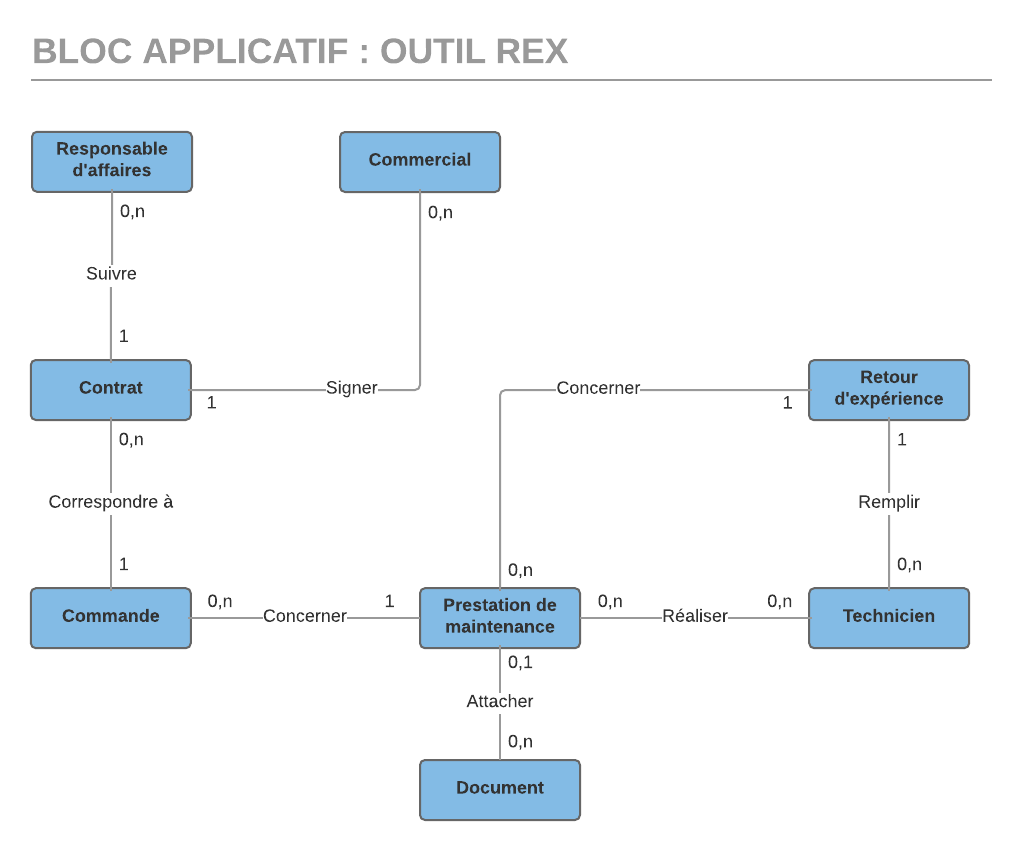
\includegraphics[width=12cm]{figures/om_rex.png}}
    \caption{Modèle Conceptuel de Données de l'outil REX}
\end{figure}

\subsubsection{Représentation de la donnée}

Afin de garantir l’efficacité la base de connaissance il sera sans doute nécessaire de mettre en place ou de réutiliser une ontologie de la maintenance. Cette base de connaissance permettra de transmettre plus efficacement l’information au sein des processus de SPIE mais aussi facilitera la tâche des techniciens et l’accès à cette dernière. Le stockage de la connaissance utilisant ce modèle permet, en effet, de proposer des résultats de recherche plus pertinents aux utilisateurs du système en intégrant les aspects sémantiques du métier. \\

Concernant l’ontologie à utiliser,  nous proposons d’utiliser l’ontologie IMAMO (Industrial MAintenance Management Ontology) qui a été formalisée par Mohamed Hedi Karray. Cette ontologie est décrite dans la figure suivante. 

\begin{figure}[H]
    \label{fig-imamo}
    \noindent\makebox[\textwidth]{
\includegraphics[width=12cm]{figures/imamo_ontology.png}}
    \caption{Vocabulaire de l'ontologie IMAMO}
\end{figure}

Cette ontologie permettra de définir classer les différentes ressources dans la base de connaissances. Il sera éventuellement nécessaire d’enrichir cette ontologie. Pour administrer cette base de connaissance on pourra utiliser Web Idea Tree\footnote{http://www.webideatree.com/} (WIT).

\subsection{Infrastructure}

Concernant l’infrastructure nécessaire pour supporter cette solution il sera nécessaire de fournir au technicien le matériel mobile équipé de l’application permettant de faire les REX. Afin de collecter les différents retours saisis par les techniciens, il sera nécessaire de mettre en place une infrastructure sous forme de serveurs de données  et d’applications. 

Les serveurs de données seront utilisés pour stocker les informations recueillies par l’application et pourront éventuellement être partagés avec les autres applications utilisées par SPIE. En effet, la mutualisation des ressources est un moyen intéressant pour réduire les dépenses si la charge des serveurs le permet.

Les serveurs d’applications pourront eux aussi être mutualisés et devront héberger l’application proposant une API pour l’application qui permet de recueillir les REX. Celle-ci devra proposer l’intégralité des services requis par l’application pour les différents cas d’utilisation.

La solution technique retenue pour développer l’application mobile pourra être Telerik\footnote{http://www.telerik.com/platform?\_ga=1.17747001.1030864250.1453189381\#overview} qui permet de développer rapidement. Concernant le “back-end” un simple serveur HTTP avec des services développés en PHP, ou technologie équivalente (NodeJS, J2E…), suffira. Pour le stockage une solution de type base de données relationnelle MySQL bien administrée conviendra.

% --------------------------- PERF
\section{Analyse des Performances (PERF)}% --------------------------- PERF
% --------------------------- PERF

\subsection{Spécifications fonctionnelles}

\subsubsection{Cas d’utilisations}

\noindent\textsc{\bf{A2 - UC1 :} Calculer le bénéfice d’un contrat}
\begin{shaded}
\noindent\textsc{Résumé :}\\

L’utilisateur consulte le dossier d’un contrat puis demande l’estimation du bénéfice associée à celui-ci, tout en estimant les potentiels risques, pouvant survenir lors de l’exécution du contrat. \\

\noindent\textsc{Utilisateur :} \\

Commercial \\

\noindent\textsc{Scénario :} \\
\begin{enumerate}
    \item L’utilisateur recherche le contrat par sa référence ou le nom de la société dans laquelle il intervient
    \item Le système affiche la liste des contrats pouvant correspondre à la recherche
    \item L’utilisateur sélectionne son contrat
    \item Le système affiche l’état actuel du contrat
    \item L’utilisateur demande l’estimation du bénéfice associé au contrat
    \item Le système calcule une estimation du bénéfice, en mettant à jour les indicateurs de performance associés au contrat.
\end{enumerate}
\end{shaded}

\noindent\textsc{\bf{A2 - UC2 :} Consulter le compte rendu des durées des prestations de maintenance d’un contrat}
\begin{shaded}
\noindent\textsc{Résumé :}\\

L’utilisateur consulte le dossier d’un contrat et demande à obtenir un compte rendu sur les durées des prestations de maintenance effectuées dans le cadre de ce contrat. \\

\noindent\textsc{Utilisateur :}\\

Responsable d’affaires \\

\noindent\textsc{Scénario :} \\
\begin{enumerate}
    \item L’utilisateur recherche le contrat par sa référence ou le nom de la société dans laquelle il intervient
    \item Le système affiche la liste des contrats pouvant correspondre à la recherche
    \item L’utilisateur sélectionne son contrat
    \item Le système affiche l’état actuel du contrat
    \item L’utilisateur demande un compte rendu sur les durées d’intervention pour ce contrat
    \item Le système lui indique la durée moyenne ainsi que les prestations de maintenance qui ont demandées le moins ainsi que le plus de temps
\end{enumerate}
\end{shaded}

\noindent\textsc{\bf{A2 - UC3 :} Consulter les statistiques d’un contrat}
\begin{shaded}
\noindent\textsc{Résumé :}\\

L’utilisateur consulte le dossier d’un contrat et demande le récapitulatif des indicateurs de performance relatifs au contrat en cours de consultation. \\

\noindent\textsc{Utilisateur :}\\

Responsable d’affaires ou Commercial \\

\noindent\textsc{Scénario :} \\
\begin{enumerate}
    \item L’utilisateur recherche le contrat par sa référence ou le nom de la société dans laquelle il intervient
    \item Le système affiche la liste des contrats pouvant correspondre à la recherche
    \item L’utilisateur sélectionne son contrat
    \item Le système affiche l’état actuel du contrat
    \item L’utilisateur demande le récapitulatif des indicateurs de performance de ce contrat
    \item Le système actualise les indicateurs et génère un rapport
\end{enumerate}
\end{shaded}

\subsubsection{Services}

\begin{description}
    \item[\textbullet] Rechercher un contrat par référence (identifiant unique) \\
        \it{Description succincte :} ce service permet de récupérer un contrat en utilisant sa référence pour la recherche. \\
        \it{Complexité :} \bf{simple}.
    \item[\textbullet] Rechercher un contrat par le nom de la société dans lequel il intervient \\
        \it{Description succincte :} ce service permet de récupérer un contrat en utilisant le nom de la société pour la recherche. \\
        \it{Complexité :} \bf{simple}.
    \item[\textbullet] Récupérer les commandes associées à une référence d’un contrat  \\
        \it{Description succincte :} ce service permet de récupérer les commandes en utilisant la référence du contrat qui leur est associé. \\
        \it{Complexité :} \bf{simple}.
    \item[\textbullet] Récupérer les prestations de maintenance associées à une référence d’une commande \\
        \it{Description succincte :} ce service permet de récupérer les prestations de maintenance en utilisant la référence de la commande associée.  \\
        \it{Complexité :} \bf{simple}.
    \item[\textbullet] Calculer l’estimation du bénéfice du contrat \\
        \it{Description succincte :} ce service permet de calculer l’estimation du bénéfice d’un contrat à partir des données du SI. \\
        \it{Complexité :} \bf{moyen}.
    \item[\textbullet] Actualiser les indicateurs de performance d’un contrat \\
        \it{Description succincte :} ce service permet d’actualiser les indicateurs du contrat à partir des informations contenues dans le SI. \\
        \it{Complexité :} \bf{moyen} à \bf{complexe}.
    \item[\textbullet] Générer un rapport sur les indicateurs du contrat \\
        \it{Description succincte :} ce service permet de générer un rapport de synthèse des indicateurs. \\
        \it{Complexité :} \bf{moyen} à \bf{complexe}.
    \item[\textbullet] Calculer la durée moyenne de toutes les prestations de maintenance d’un contrat \\
        \it{Description succincte :} ce service permet de calculer, à partir des données du SI, la durée moyenne des prestations de maintenance. \\
        \it{Complexité :} \bf{moyen}.
    \item[\textbullet] Récupérer les prestations de maintenance qui ont demandées le plus de temps \\
        \it{Description succincte :} ce service permet de récupérer les prestations de maintenance qui ont durée le plus longtemps en utilisant un seuil minimal. \\
        \it{Complexité :} \bf{moyen}.
    \item[\textbullet] Récupérer les prestations de maintenance qui ont demandées le moins de temps \\
        \it{Description succincte :} ce service permet de récupérer les prestations de maintenance qui ont durée le moins longtemps en utilisant un seuil maximal. \\
        \it{Complexité :} \bf{moyen}.
\end{description}

\subsubsection{Identification du bloc applicatif}

Le bloc applicatif “Outil PERF” permet de regrouper les différents services répondant aux cas d’utilisation liés à la mise en place des indicateurs de performance et la standardisation des processus liés. Ce bloc doit également interagir avec une base de données et c’est pourquoi cet acteur apparaît sur le schéma ci-dessous. D’un point de vue humain, seuls les commerciaux et les responsables d’affaires sont concernés par cet outil qui exploitent également les données issues de l’outil REX précédemment introduit.

\begin{figure}[H]
    \label{fig-uc-perf}
    \noindent\makebox[\textwidth]{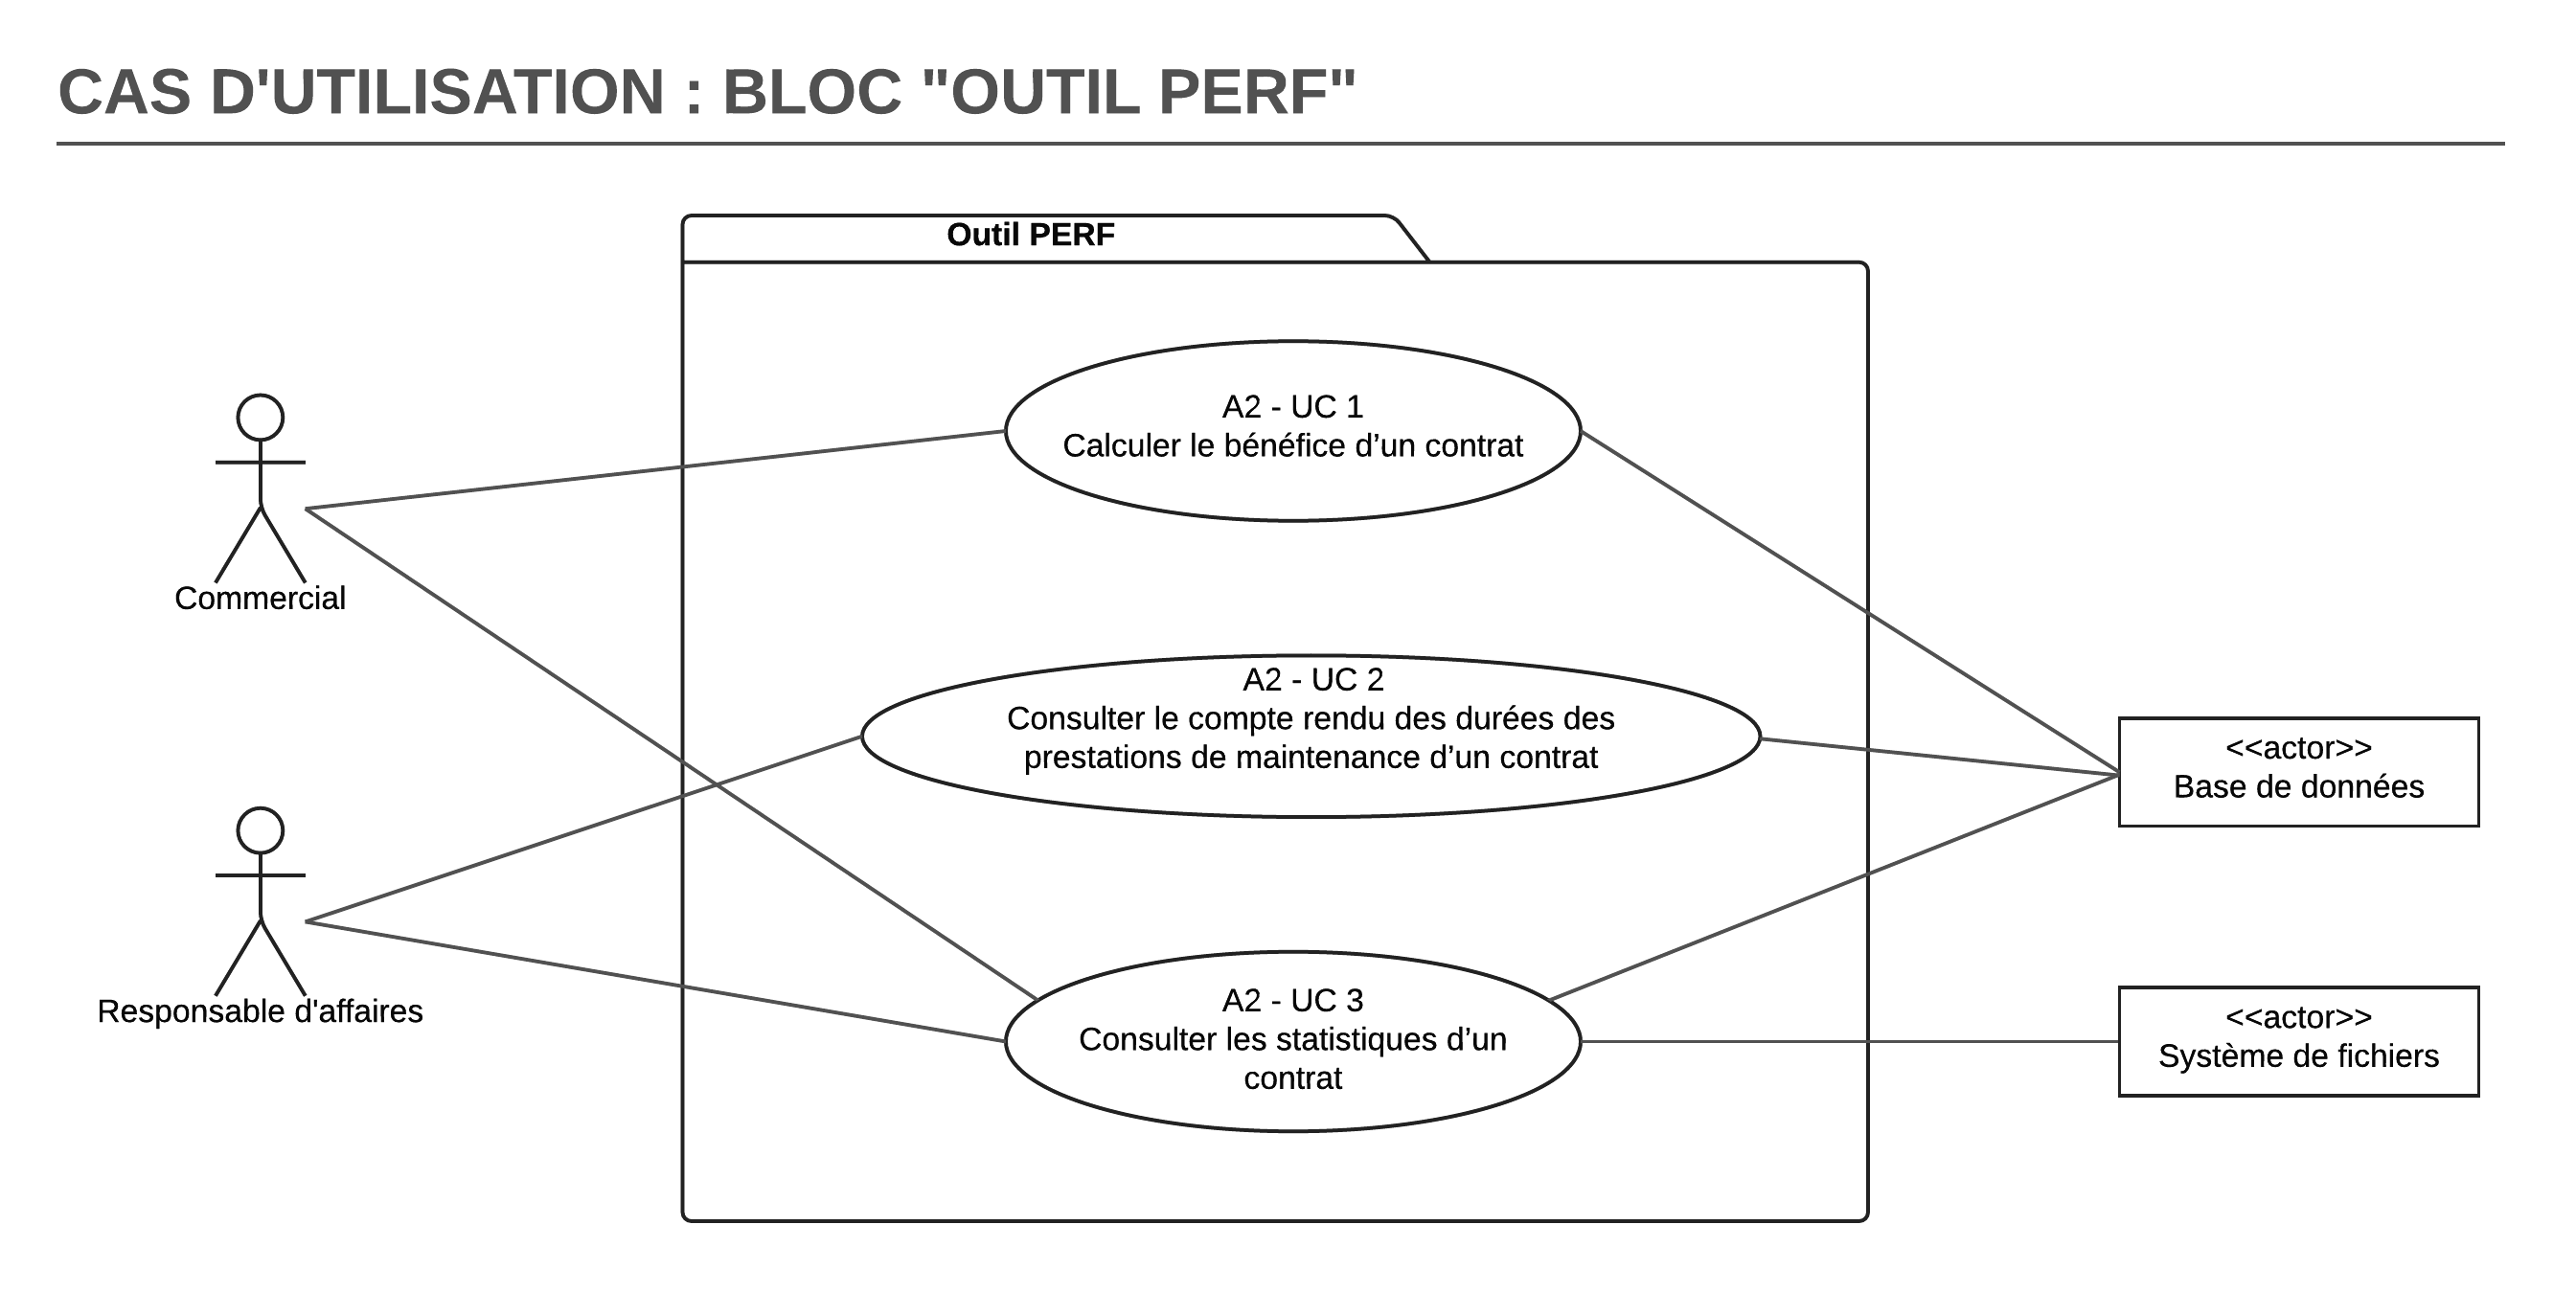
\includegraphics[width=12cm]{figures/uc_bloc_perf.png}}
    \caption{Diagramme des cas d'utilisation de l'outil PERF}
\end{figure}

Les dépendances du bloc “Outil PERF” vis à vis des blocs existant et des nouveaux blocs sont décrites dans le schéma suivant. Celles-ci sont nombreuses et traduisent les besoins tels que la communication avec “Calrify” pour la récupération des données de maintenance mais aussi les outils “ADV” et “SUPRA” concernant respectivement les informations relatives aux ventes et aux responsables d’affaires. Pour finir, ce bloc nécessite aussi la prise en compte des nouvelles informations apportées par le bloc “Outil REX” introduit dans la partie précédente.

\begin{figure}[H]
    \label{fig-dep-perf}
    \noindent\makebox[\textwidth]{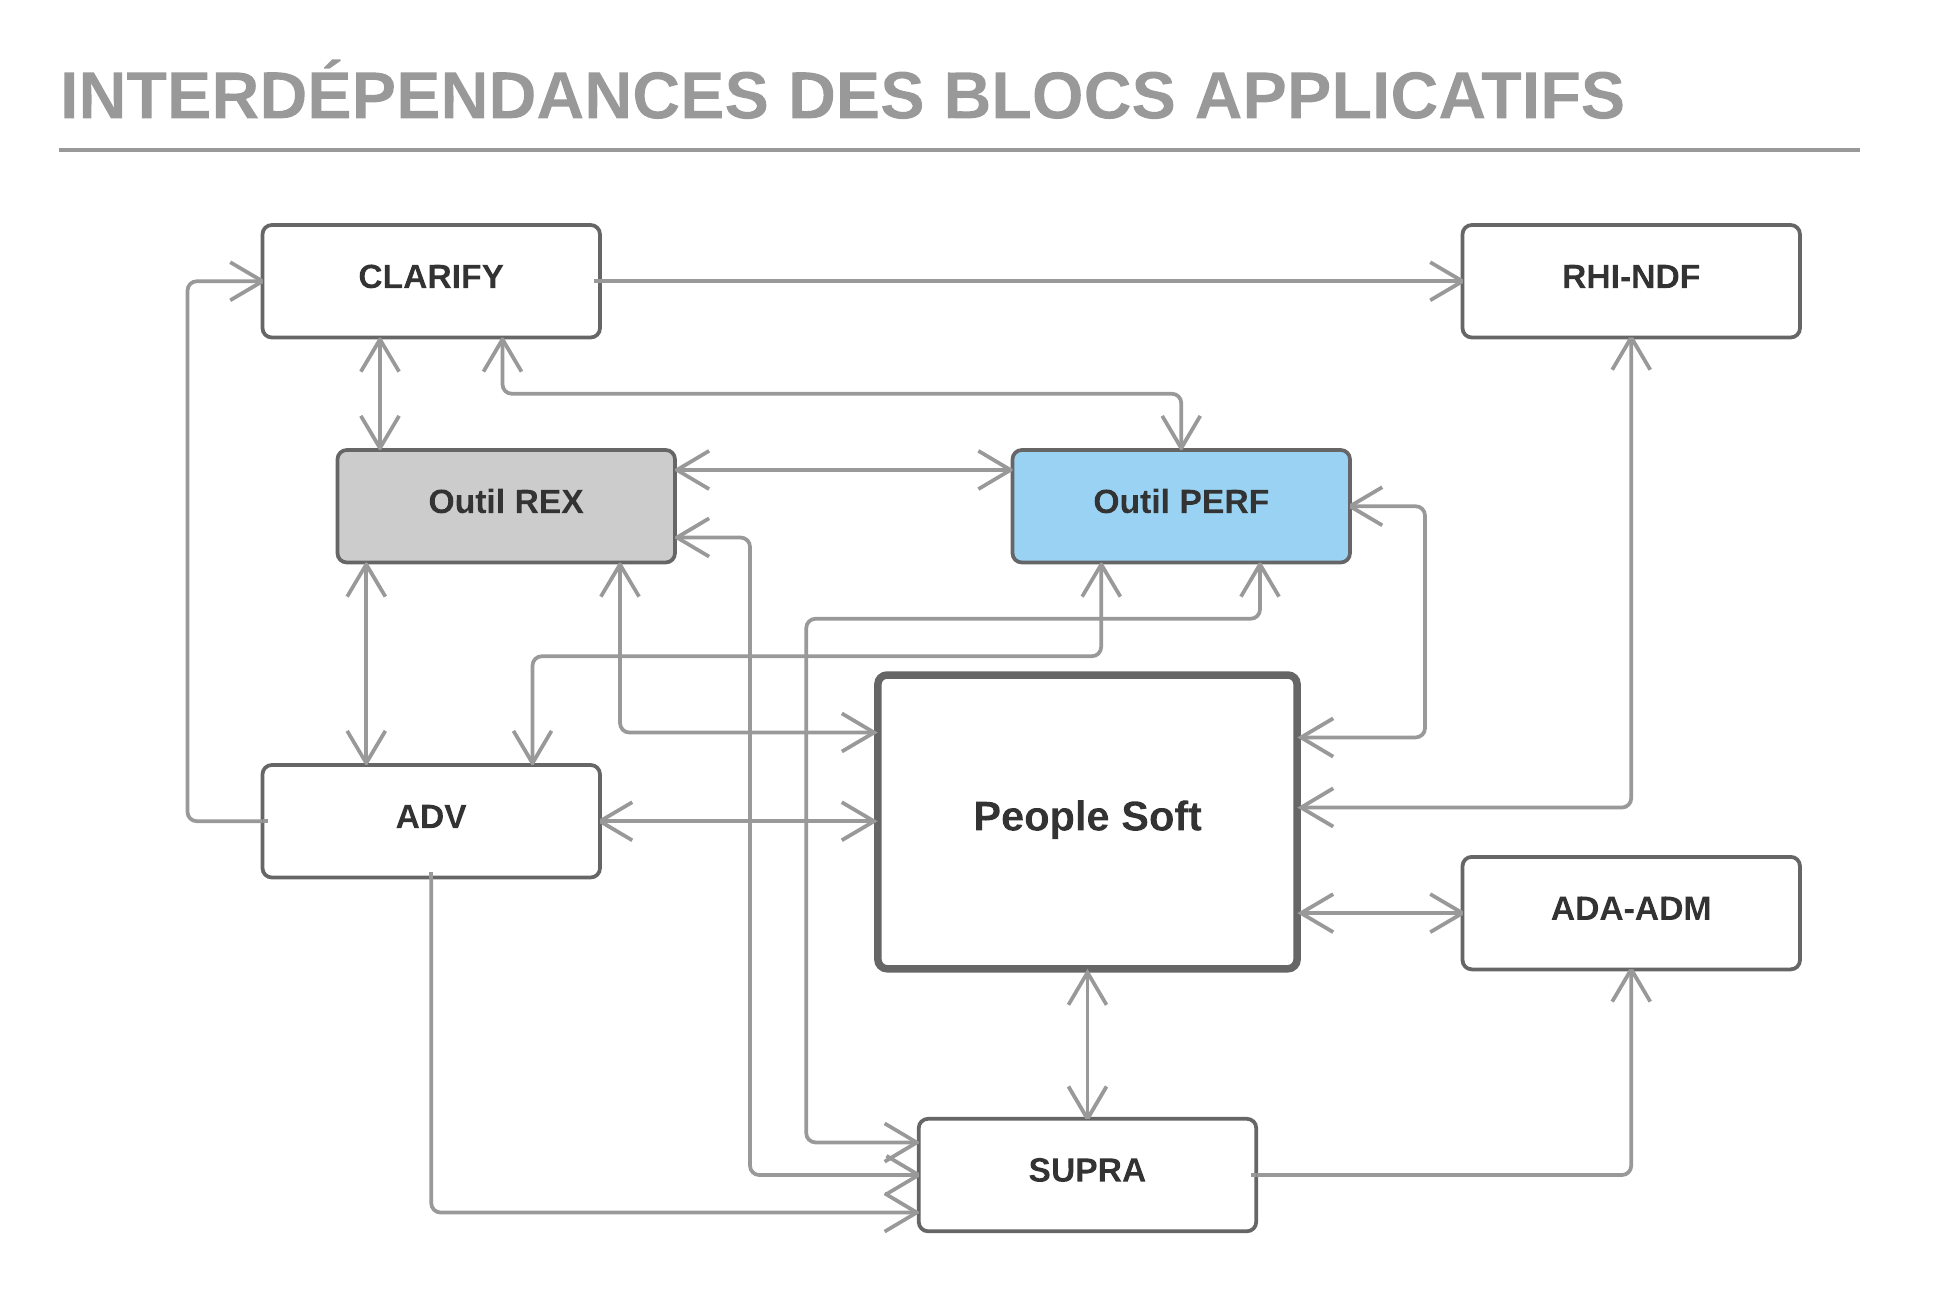
\includegraphics[width=12cm]{figures/dependances_bloc_perf.png}}
    \caption{Schéma des interdépendances de l'outil PERF}
\end{figure}

\subsection{Gestion des données}

\subsubsection{Objets métiers}

Les différents cas d’utilisation décrits précédemment permettent d’identifier les objets métiers qui sont concernés par ceux-ci, permettant dans le même temps de compléter le modèle conceptuel de données correspondant à la solution spécifique proposée.

\begin{table}[H]
    \begin{tabular}{p{3cm}|p{10cm}|p{3cm}}
    Objet métier & Description & Cas d'utilisations \\ \hline
    Contrat & Contrat de maintenance signé par un client de SPIE Sud-Est & A2 - UC1 ; A2 - UC2 ; A2 - UC3 \\ \hline
    Commande & Commande de la part d’un client d’un ensemble de prestations de maintenance, dans le cadre d’un contrat de maintenance & A2 - UC1 ; A2 - UC2 ; A2 - UC3 \\ \hline
    Prestation de maintenance & Intervention de maintenance effectuée par un technicien pour un client
 & A2 - UC2 ; A2 - UC3 \\ \hline
    Commercial & Commercial signant les contrats de maintenance & A2 - UC1 ; A2 - UC3 \\ \hline
    Responsable d’affaires & Responsable d’affaires suivant le déroulement des contrats de maintenance & A2 - UC2 ; A2 - UC3 \\ 
    \end{tabular}
    \caption{Tableau des Objets Métiers pour l'Outil PERF}
\end{table}

Le bloc applicatif “Outil PERF” utilisant ces différents objets métier, leurs relations peuvent être modélisées selon le modèle conceptuel de données ci-dessous.

\begin{figure}[H]
    \label{fig-om-perf}
    \noindent\makebox[\textwidth]{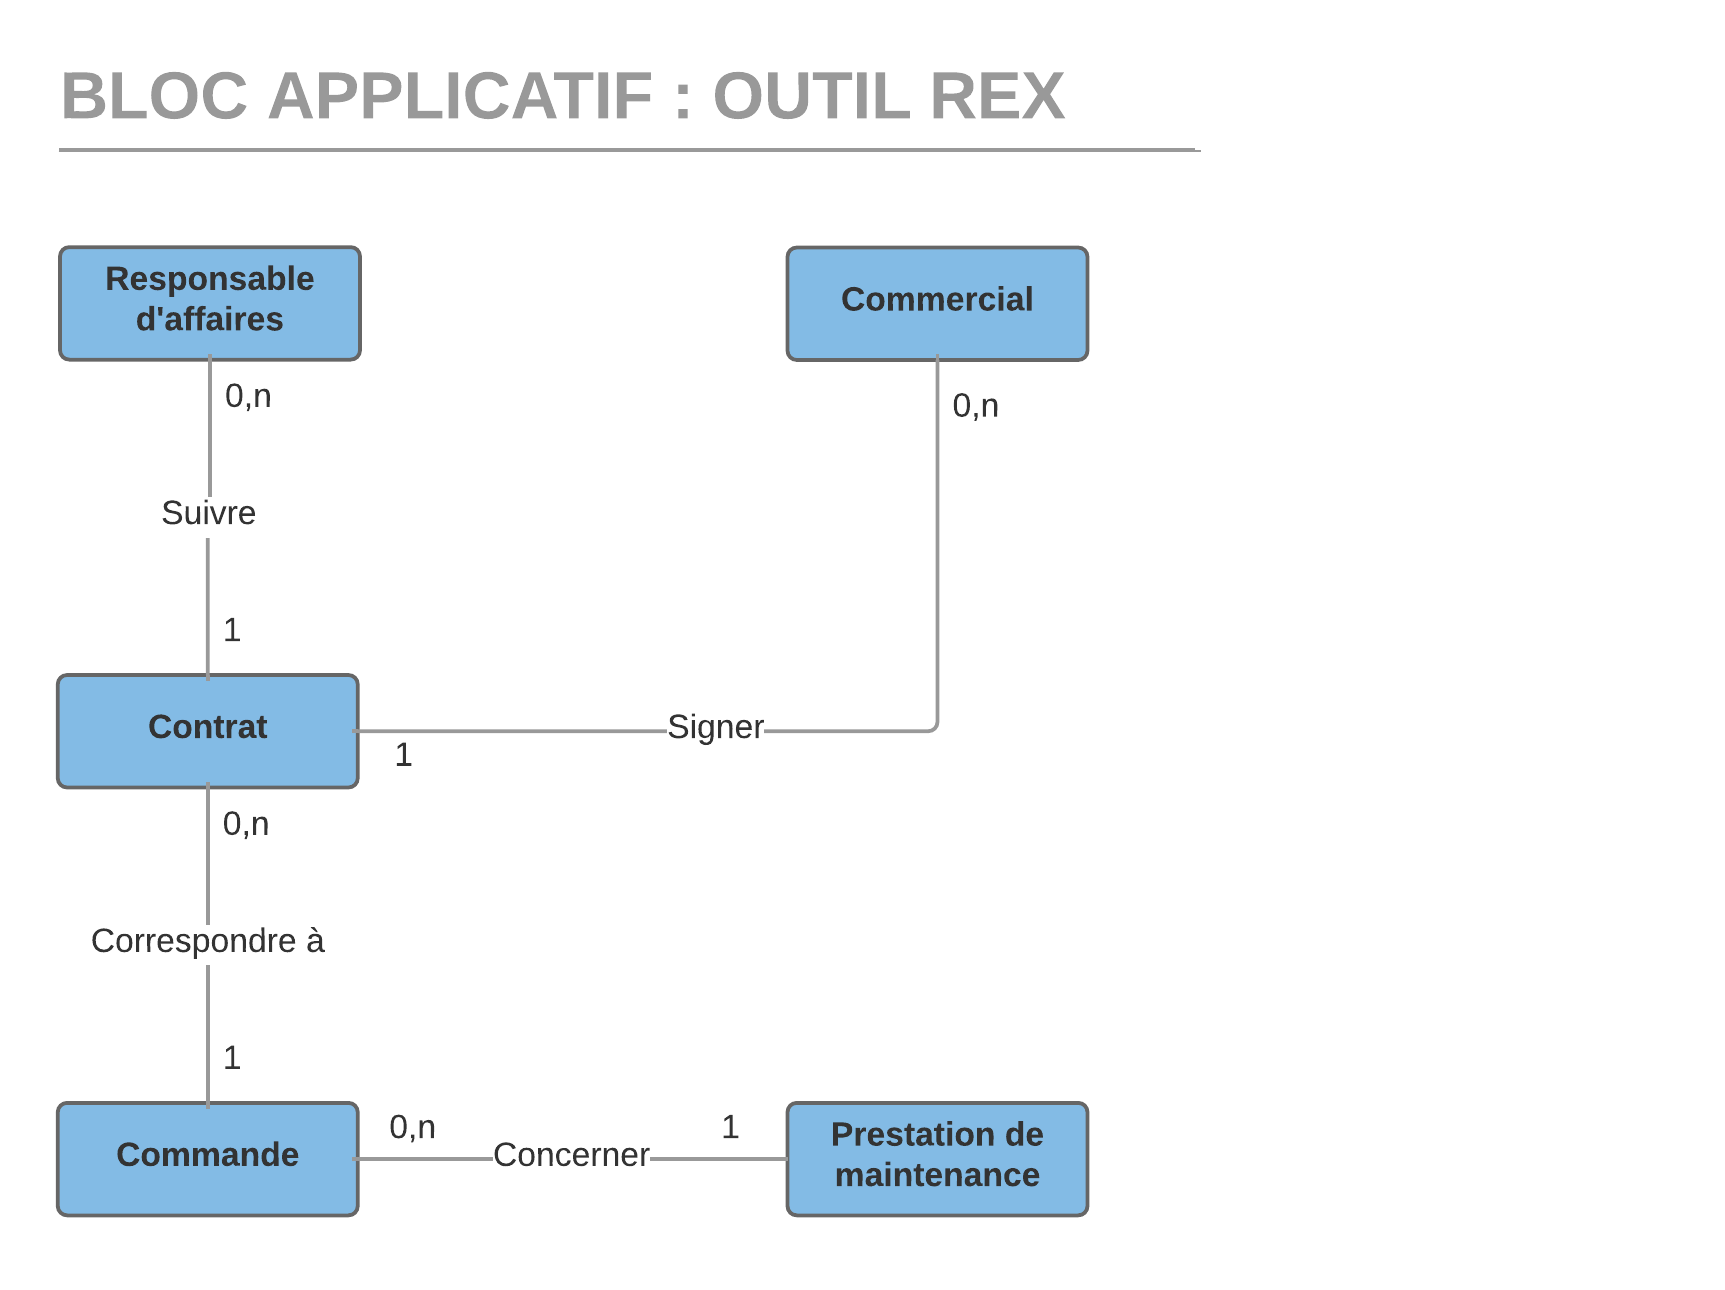
\includegraphics[width=12cm]{figures/om_perf.png}}
    \caption{Modèle Conceptuel de Données de l'outil PERF}
\end{figure}

\subsubsection{Représentation de la donnée}

Toutes les données stockées concernant les contrats devront pouvoir être accessible par l’application qui sera chargée d’agréger ces données pour réaliser des statistiques qui alimenteront les différents tableaux de bord. La mise en place d’un entrepôt de données alimenté par les autres applicatifs doit être envisagé pour aller dans ce sens. \\

Il sera également nécessaire de concevoir les hypercubes associés afin de pouvoir exploiter ces données. Pour parvenir à ce résultat, SPIE devra faire l’acquisition des outils permettant de manipuler ces données, Pentaho par exemple. 

\subsection{Infrastructure}

Le stockage des données nécessitera une infrastructure conséquente garantissant une bonne qualité de service et permettant éventuellement des opérations de réplication pour protéger SPIE d’une perte importante de données. \\

Les dispositions à prendre pour mettre en place une telle infrastructure sont les suivantes : acquérir plusieurs serveurs de données et les configurer de sorte à mettre en place la réplication. Concernant la localisation de ces serveurs, il serait judicieux de les placer dans divers endroits si possible avec des alimentations électriques distinctes et redondantes. 

% --------------------------- RISQUE
\section{Analyse des Risques (RISQUE)}% --------------------------- RISQUE
% --------------------------- RISQUE

\subsection{Spécifications fonctionnelles}

\subsubsection{Cas d’utilisations}

\noindent\textsc{\bf{A3 - UC1 :} Calculer l’indice de niveau de sécurité}
\begin{shaded}
\noindent\textsc{Résumé :}\\

Lors de la mise à jour des informations relatives à un contrat ou à une intervention, l’indice de niveau de sécurité est recalculé en intégrant les nouvelles données. \\

\noindent\textsc{Utilisateur :} \\

Commercial ou Responsable d’affaires \\

\noindent\textsc{Scénario :} \\
\begin{enumerate}
    \item L’utilisateur recherche le contrat par sa référence ou le nom de la société dans laquelle il intervient
    \item Le système affiche la liste des contrats pouvant correspondre à la recherche
    \item L’utilisateur sélectionne son contrat
    \item Le système affiche l’état actuel du contrat
    \item L’utilisateur demande le calcul de l’indice de niveau de sécurité du contrat
    \item Le système recalcule l’indice de niveau de sécurité et l’indique à l’utilisateur
\end{enumerate}
\end{shaded}

\noindent\textsc{\bf{A3 - UC2 :} Estimer le niveau de risque d’un contrat}
\begin{shaded}
\noindent\textsc{Résumé :}\\

Lors de la mise à jour des informations relatives à un contrat, le niveau de risque est recalculé en intégrant les nouvelles données. \\

\noindent\textsc{Utilisateur :} \\

Commercial ou Responsable d’affaires \\

\noindent\textsc{Scénario :} \\
\begin{enumerate}
    \item L’utilisateur recherche le contrat par sa référence ou le nom de la société dans laquelle il intervient
    \item Le système affiche la liste des contrats pouvant correspondre à la recherche
    \item L’utilisateur sélectionne son contrat
    \item Le système affiche l’état actuel du contrat
    \item L’utilisateur demande le niveau de risque du contrat
    \item Le système recalcule le niveau de risque et l’indique à l’utilisateur
\end{enumerate}
\end{shaded}

\noindent\textsc{\bf{A3 - UC3 :} Rechercher une solution à un problème référencé}
\begin{shaded}
\noindent\textsc{Résumé :}\\

L’utilisateur souhaite trouver une solution à un problème qu’il suppose référencé dans la base de connaissance. \\

\noindent\textsc{Utilisateur :} \\

Technicien ou Responsable d’affaires \\

\noindent\textsc{Scénario :} \\
\begin{enumerate}
    \item L’utilisateur saisit des mots clés qui décrivent son problème
    \item Une liste de solutions contenant les mots clés est présentée à l’utilisateur
    \item L’utilisateur peut consulter le contenu des différentes solutions afin de trouver une réponse à sa problématique \\
\end{enumerate}
\noindent\textsc{Scénarii alternatifs :}\\
\begin{enumerate}
    \item Aucune solution ne comporte les mots clés saisis et le système ne connaît apparemment pas de réponse à ce problème.
    \item L’utilisateur peut demander la création d’une solution dans la base de connaissance relatif à ce problème et proposer une résolution au problème une fois que celui-ci a été résolu.
\end{enumerate}
\end{shaded}

\subsubsection{Services}

\begin{description}
    \item[\textbullet] Rechercher un contrat par référence (identifiant unique) \\
        \it{Description succincte :} ce service permet de récupérer un contrat en utilisant sa référence pour la recherche. \\
        \it{Complexité :} \bf{simple}.
    \item[\textbullet] Rechercher un contrat par le nom de la société dans lequel il intervient \\
        \it{Description succincte :} ce service permet de de récupérer un contrat de maintenance en utilisant le nom de la société pour la recherche. \\
        \it{Complexité :} \bf{simple}.
    \item[\textbullet] Calculer l’indice de niveau de sécurité du contrat \\
        \it{Description succincte :} ce service permet de calculer l’indice de niveau de sécurité à partir des informations présentes dans le SI. \\
        \it{Complexité :} \bf{complexe}.
    \item[\textbullet] Calculer l’indice de risque du contrat \\
        \it{Description succincte :} ce service permet de calculer l’indice de risque à partir des informations présentes dans le SI. \\
        \it{Complexité :} \bf{complexe}.
    \item[\textbullet] Rechercher une solution par des mots-clés \\
        \it{Description succincte :} ce service permet de récupérer des solutions contenant des mots-clés ou liées à des concepts présent dans la recherche. \\
        \it{Complexité :} \bf{moyen} à \bf{complexe}.
    \item[\textbullet] Rechercher une solution par son identifiant \\
        \it{Description succincte :} ce service permet de récupérer une solution en utilisant son identifiant pour effectuer la rechercher. \\
        \it{Complexité :} \bf{simple}.
    \item[\textbullet] Créer une nouvelle solution à un problème \\
        \it{Description succincte :} ce service permet d’éditer une nouvelle solution à un problème répertorié en exploitant les saisies de l’utilisateur. \\
        \it{Complexité :} \bf{moyen}.
    \item[\textbullet] Modifier une solution présente dans la base de connaissance \\
        \it{Description succincte :} ce service permet de modifier une solution précédemment ajoutée \\
        \it{Complexité :} \bf{moyen}.
\end{description}

\subsubsection{Identification du bloc applicatif}

Le bloc “Outil RISQUE”, comme les deux précédents, requiert un accès à la base de données pour mettre à jour les indices qu’il permet de calculer. Il doit également pouvoir accéder aux informations alimentant ces calculs. Le schéma intitulé “Cas d’Utilisation : Bloc “Outil RISQUE”” présente donc l’acteur base de données. Ce bloc concerne tous les utilisateurs, c’est-à-dire les commerciaux, les responsables d’affaires et les techniciens car il propose un panel de fonctionnalités relativement large.

\begin{figure}[H]
    \label{fig-uc-risque}
    \noindent\makebox[\textwidth]{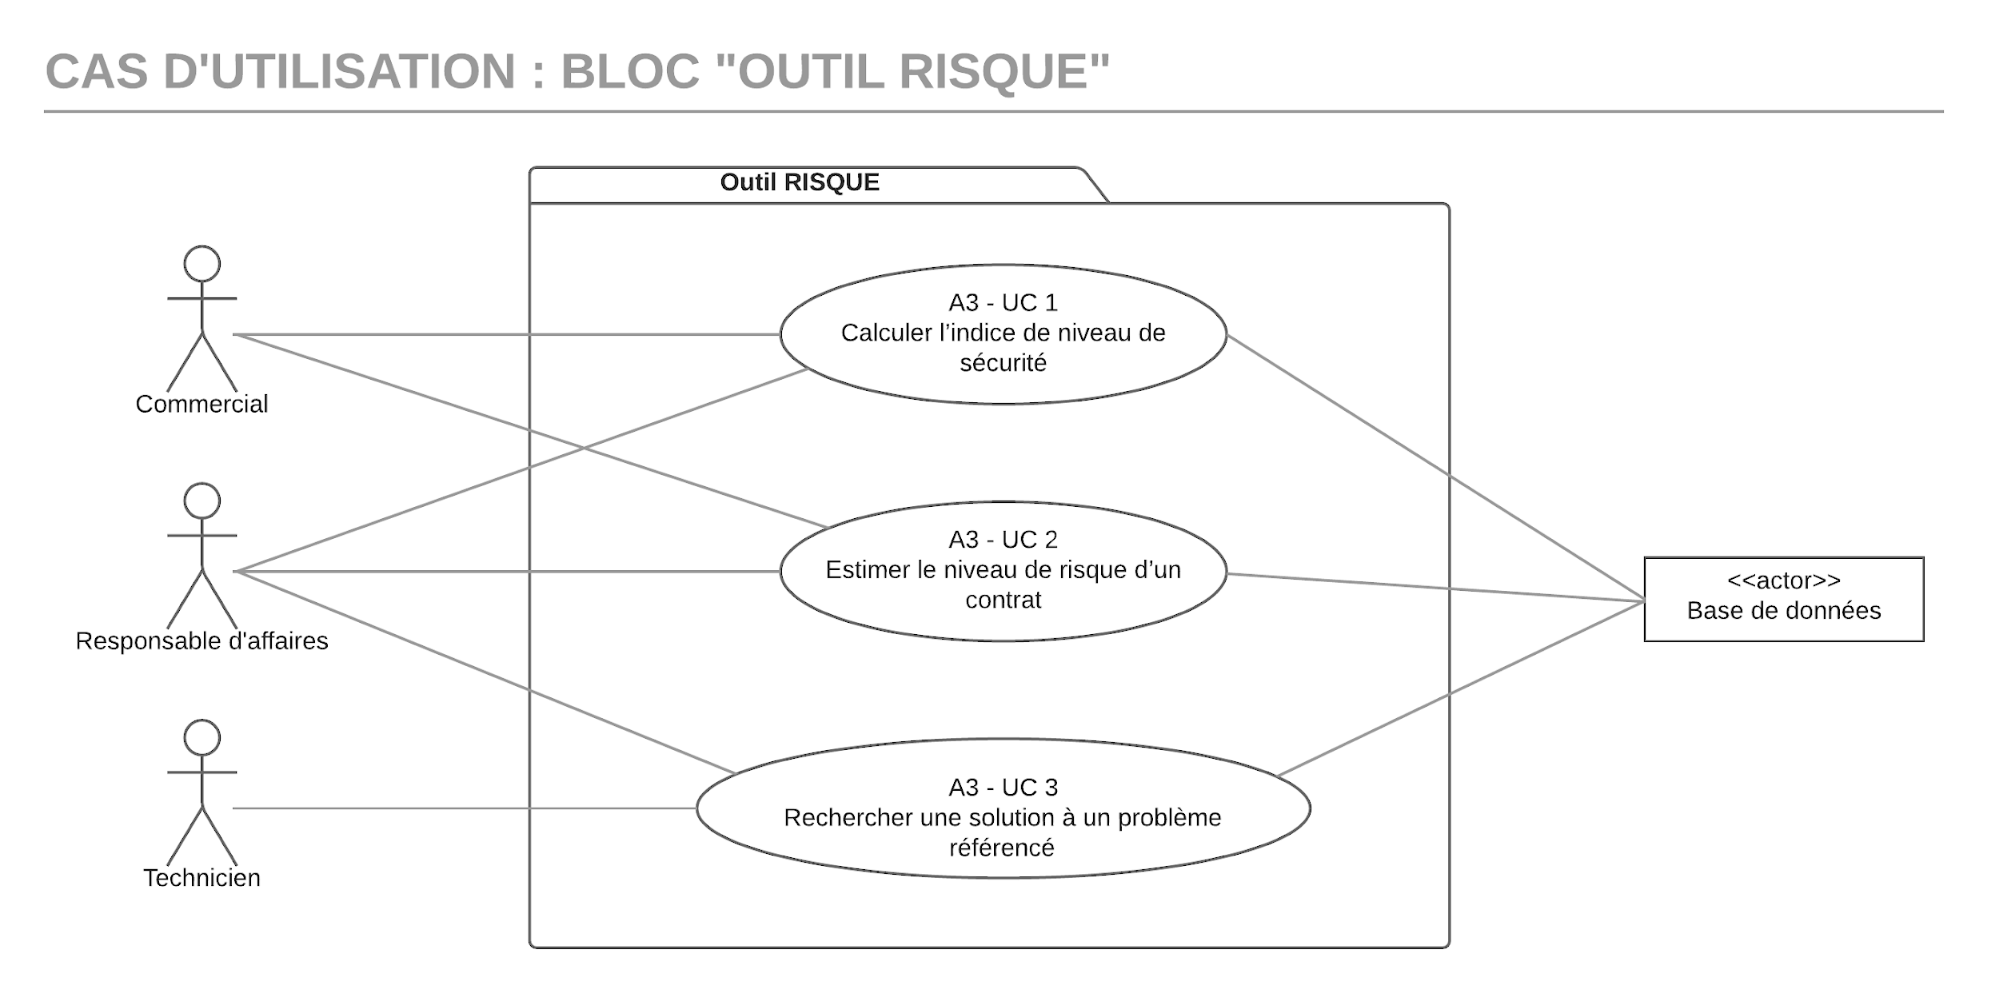
\includegraphics[width=12cm]{figures/uc_bloc_risque.png}}
    \caption{Diagramme des cas d'utilisation de l'outil RISQUE}
\end{figure}

Concernant la communication de du bloc “Outil RISQUE” avec les blocs existant et les deux blocs introduits précédemment nous constatons que les liens sont similaires. En effet, ce module requiert des informations provenant des autres blocs et notamment des connaissances recueillies auprès des différents acteurs humains par le biais des outils. Il est important de noter que cela se répercutera également sur l’architecture applicative et l’infrastructure à développer. Certains éléments de ces architectures pourrons évidemment être mutualisés pour répondre au besoin. La mutualisation présente de nombreux avantages, en particulier sur le plan financier.

\begin{figure}[H]
    \label{fig-dep-risque}
    \noindent\makebox[\textwidth]{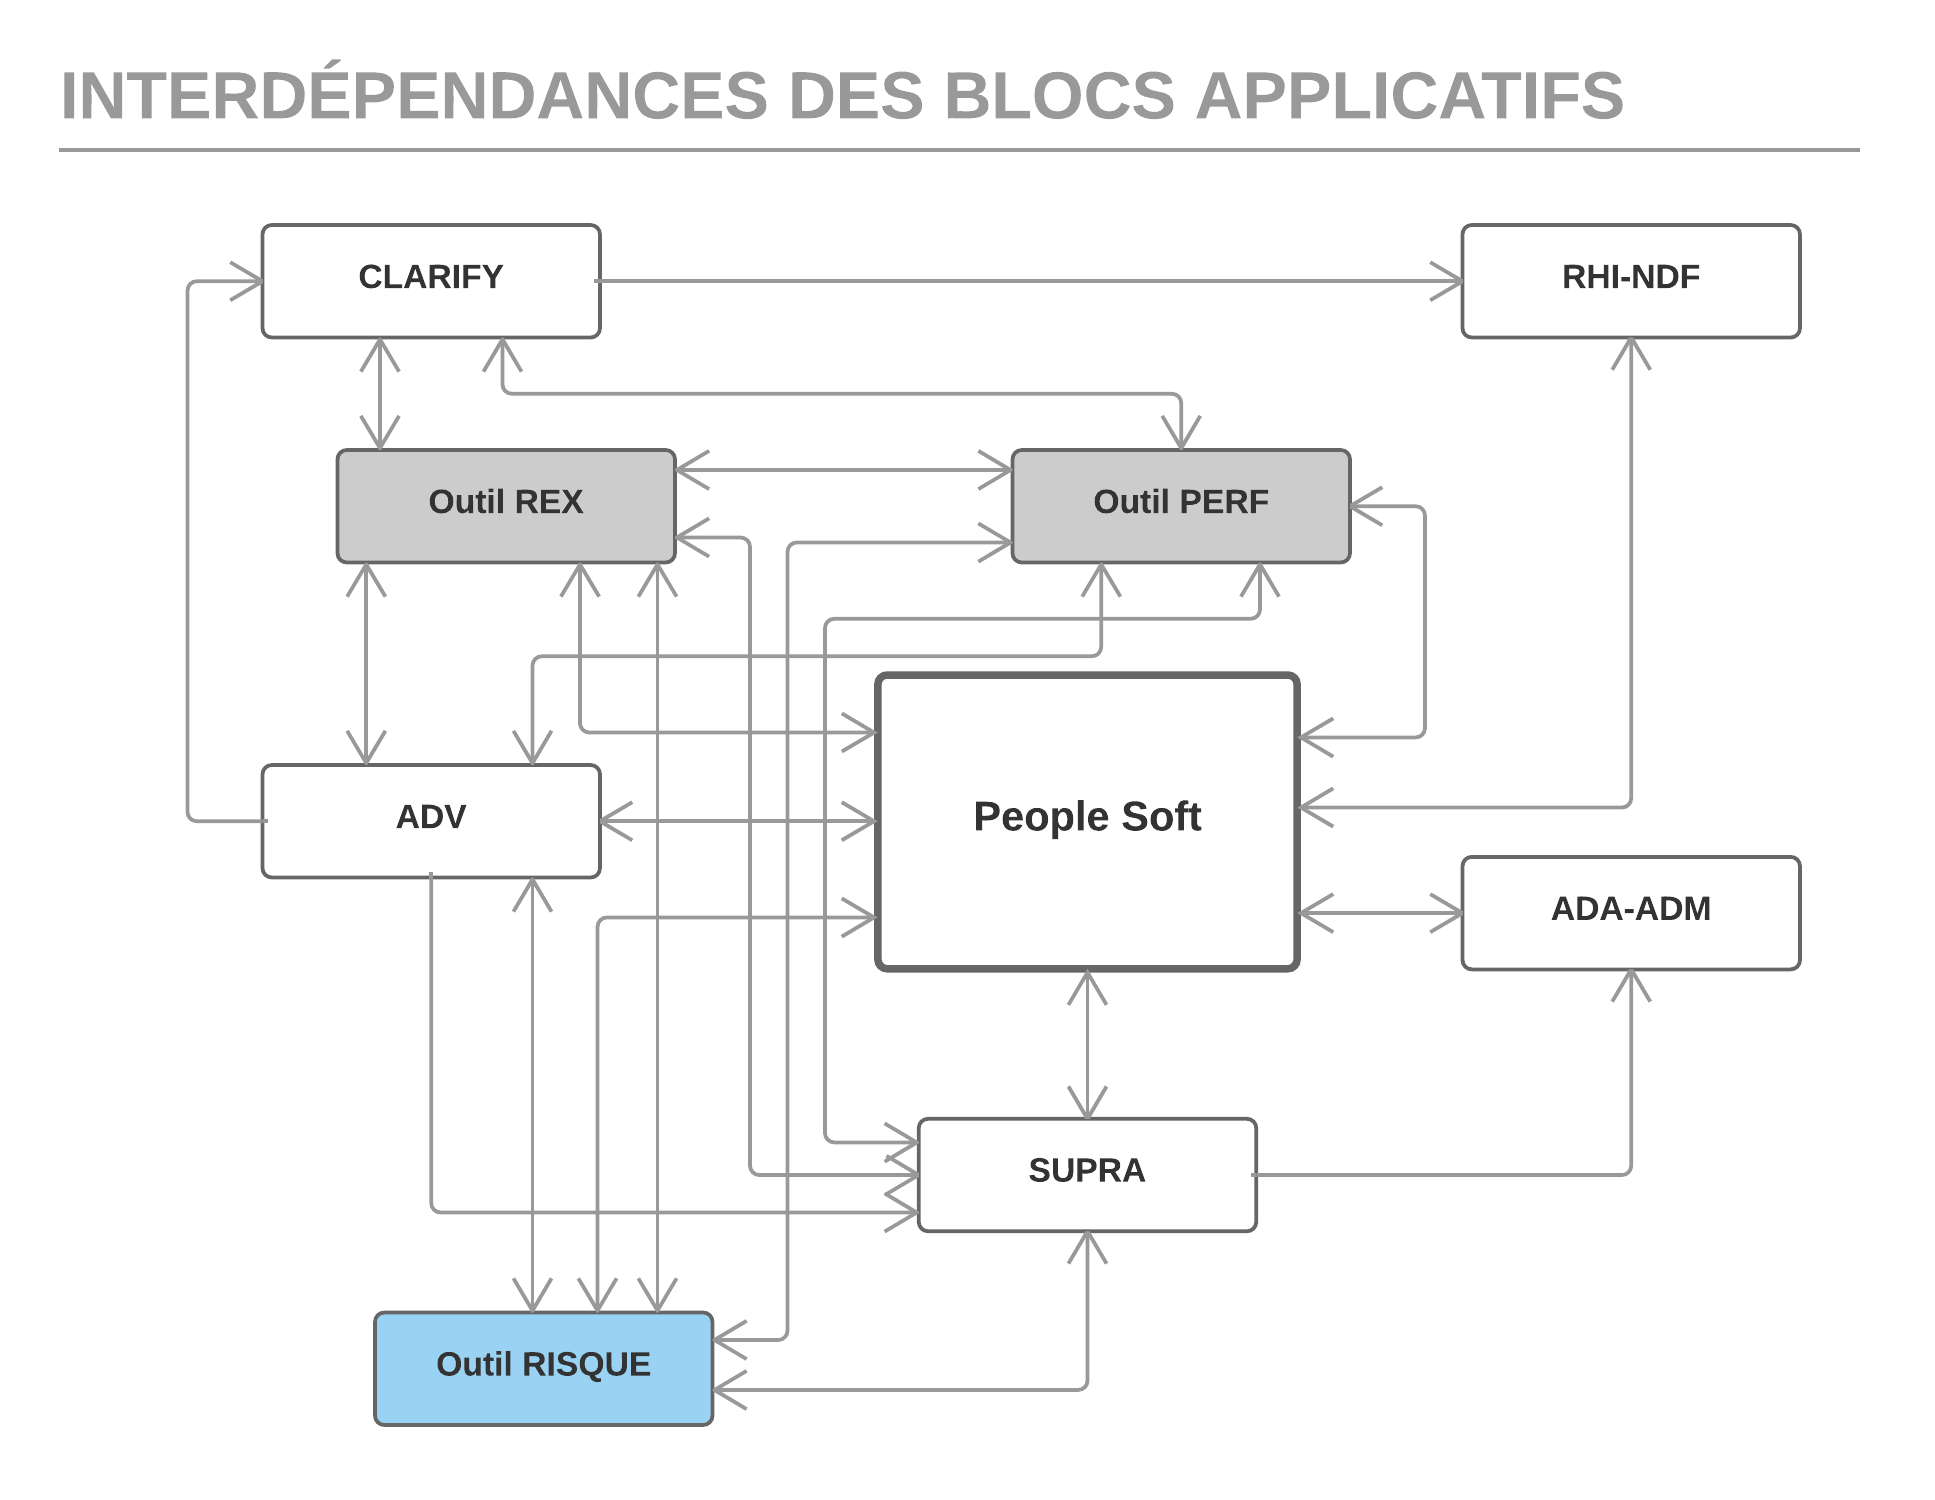
\includegraphics[width=12cm]{figures/dependances_bloc_risque.png}}
    \caption{Schéma des interdépendances de l'outil RISQUE}
\end{figure}

\subsection{Gestion des données}

\subsubsection{Objets métiers}

Les différents cas d’utilisation décrits précédemment permettent d’identifier les objets métiers qui sont concernés par ceux-ci. Permettant aussi de compléter le modèle conceptuel de données correspondant à la solution spécifique proposée.

\begin{table}[H]
    \begin{tabular}{p{3cm}|p{10cm}|p{3cm}}
    Objet métier & Description & Cas d'utilisations \\ \hline
    Contrat & Contrat de maintenance signé par un client de SPIE Sud-Est & A3 - UC1 ; A3 - UC2 \\ \hline
    Commande & Commande de la part d’un client d’un ensemble de prestations de maintenance, dans le cadre d’un contrat de maintenance & A3 - UC1 ; A3 - UC2 \\ \hline
    Prestation de maintenance & Intervention de maintenance effectuée par un technicien pour un client & A3 - UC1 ; A3 - UC2 \\ \hline
    Retour d’expérience & Compte-rendu effectué par un technicien après une prestation de maintenance & A3 - UC3 \\ \hline
    Commercial & Commercial signant les contrats de maintenance & A3 - UC1 ; A3 - UC2 \\ \hline
    Responsable d’affaires & Responsable d’affaires suivant le déroulement des contrats de maintenance & A3 - UC1 ; A3 - UC3 \\ \hline
    Technicien & Technicien réalisant les prestations de maintenance & A3 - UC3 \\
    \end{tabular}
    \caption{Tableau des Objets Métiers pour l'Outil RISQUE}
\end{table}

Le bloc applicatif “Outil RISQUE” utilisant ces différents objets métier, leurs relations peuvent être modélisée selon le modèle conceptuel de données ci-dessous.

\begin{figure}[H]
    \label{fig-om-risque}
    \noindent\makebox[\textwidth]{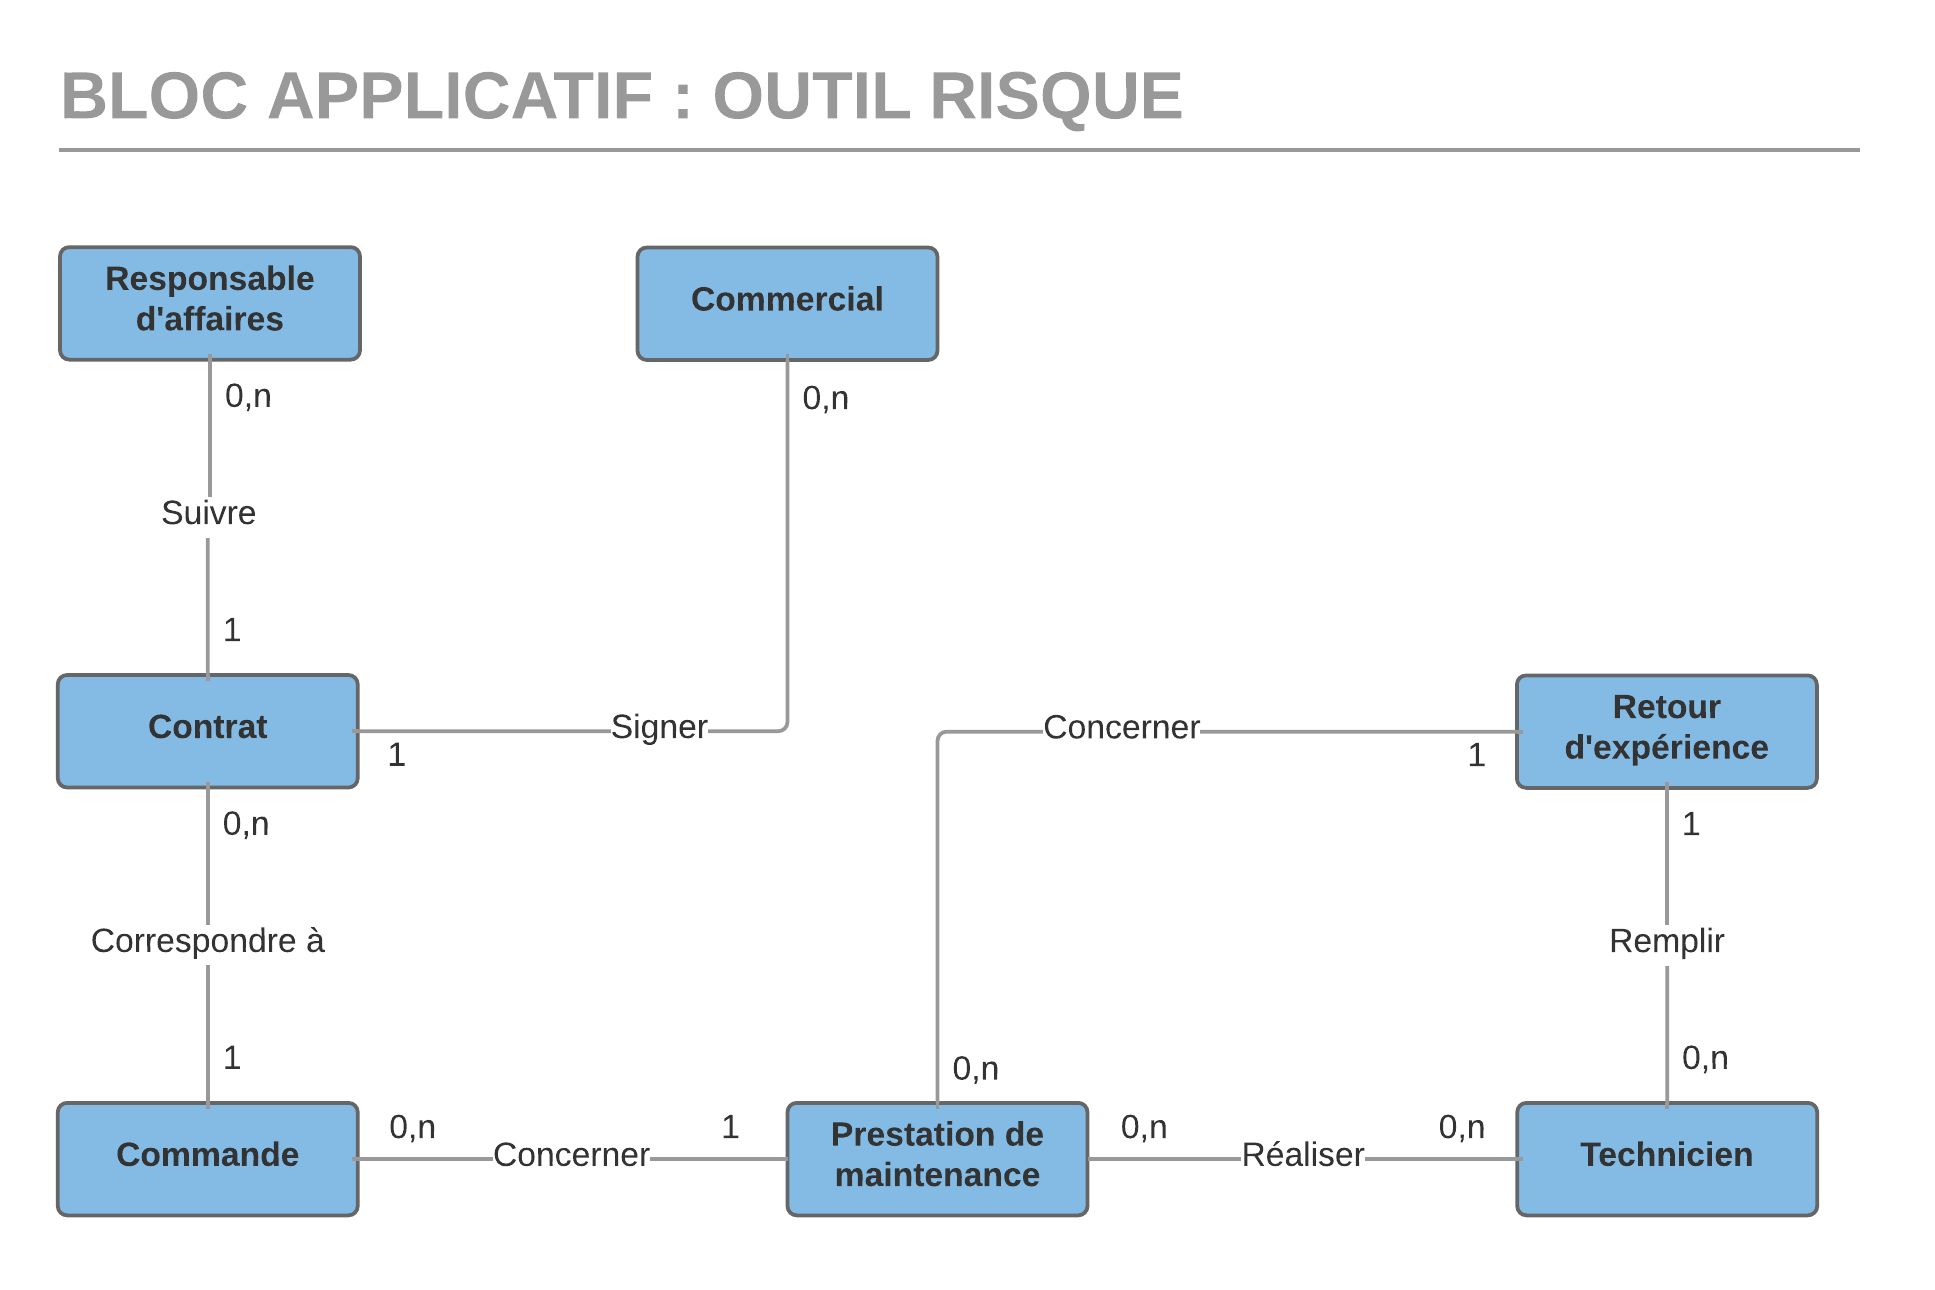
\includegraphics[width=12cm]{figures/om_risque.png}}
    \caption{Modèle Conceptuel de Données de l'outil RISQUE}
\end{figure}

\subsubsection{Représentation de la donnée}

Du point de vue de la gestion des données, celle-ci est étroitement liée à l’axe concernant les REX. En effet, la prédiction des risques nécessite de se baser sur des connaissances accumulées au cours des différentes activités menées dans le cadre de ces projets pour anticiper, dans la mesure du possible, les problèmes qui peuvent être rencontrés lors du déroulement de projet.

Nous conseillons donc de vous reporter au paragraphe correspondant dans la section de l’axe d’amélioration associé.

\subsection{Infrastructure}

Cette solution nécessite de mettre en place une interface simple permettant d’accéder facilement à l’ensemble des connaissances répertoriées dans cette base. Cette interface pourrait s’appuyer sur une application web hébergée sur un des serveurs d’application de SPIE Sud-Est. Ce serveur pourra être un serveur mutualisé.
